%!TEX root = ../paper.tex
This section presents a visual representation of the results of the estimators that allows us to compare the performance of the two estimators on a single dataset. All plots associated with a single dataset have the same axes. The horizontal axis is used to represent the known densities, this axis has the same range as the known densities. The estimated densities are shown on the vertical axis, the length of these axes is such that they are long enough to represent every estimated density for that dataset, independent of the used estimator. The black line in each plot illustrates the line all points would lie on if a perfect estimator was used, \ie the line $x = x$. The colors of the points in these plot correspond to the colors of the elements of the datasets in \cref{tab:3:simulated:datasets} and \cref{fig:3:simulated:datasets}.

% Single Sphere Data
	\begin{figure*}
		\centering
		%!TEX root = ../paper.tex

\begin{figure*}
	\centering
	%!TEX root = ../paper.tex

% Ferdosi 1 - MBE
\begin{subfigure}{0.23\textwidth}
	\centering
	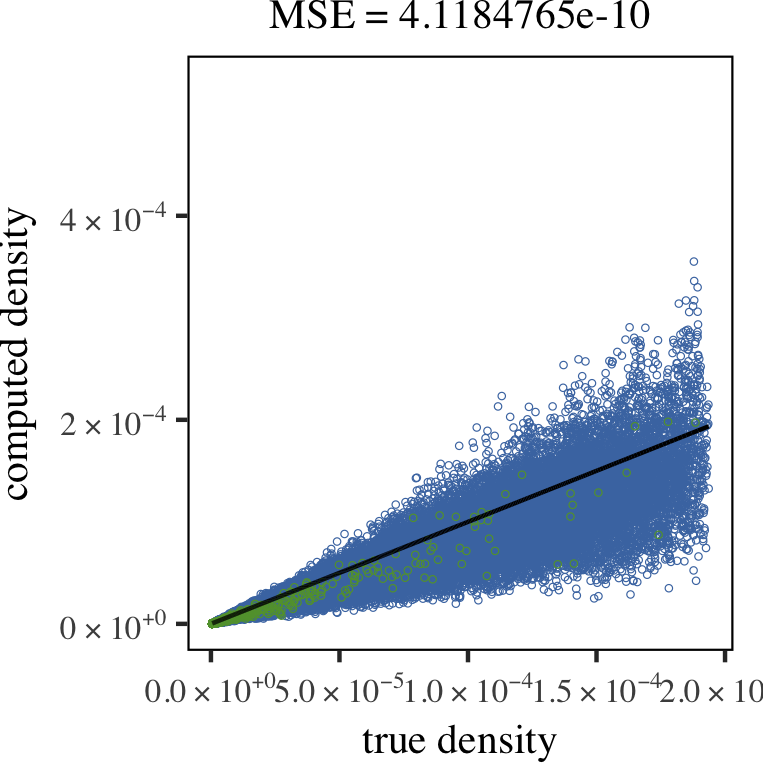
\includegraphics[keepaspectratio=true, width=\textwidth, height=0.23\textheight]{result/img/all/results_ferdosi_1_60000_mbe_silverman}
	\caption{Set \ferdosiOne, \mbe}
	\label{fig:4:results:mbe:ferdosi1}
\end{subfigure}
% Baakman 1	- MBE
\begin{subfigure}{0.23\textwidth}
	\centering
	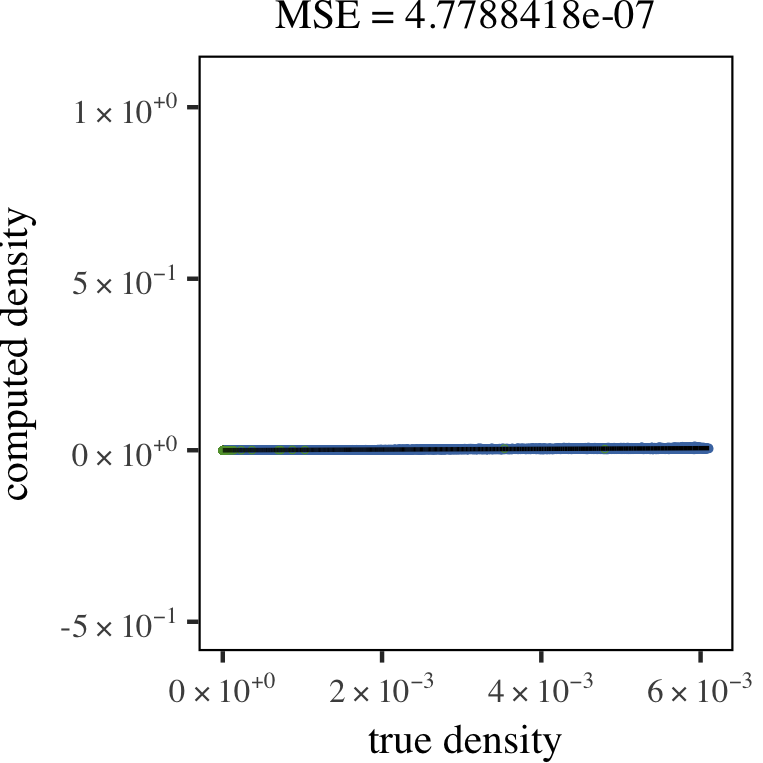
\includegraphics[keepaspectratio=true, width=\textwidth, height=0.23\textheight]{result/img/all/results_baakman_1_60000_mbe_silverman}
	\caption{Set \baakmanOne, \mbe}
	\label{fig:4:results:mbe:baakman1}
\end{subfigure}
% Baakman 4 - MBE
\begin{subfigure}{0.23\textwidth}
	\centering
	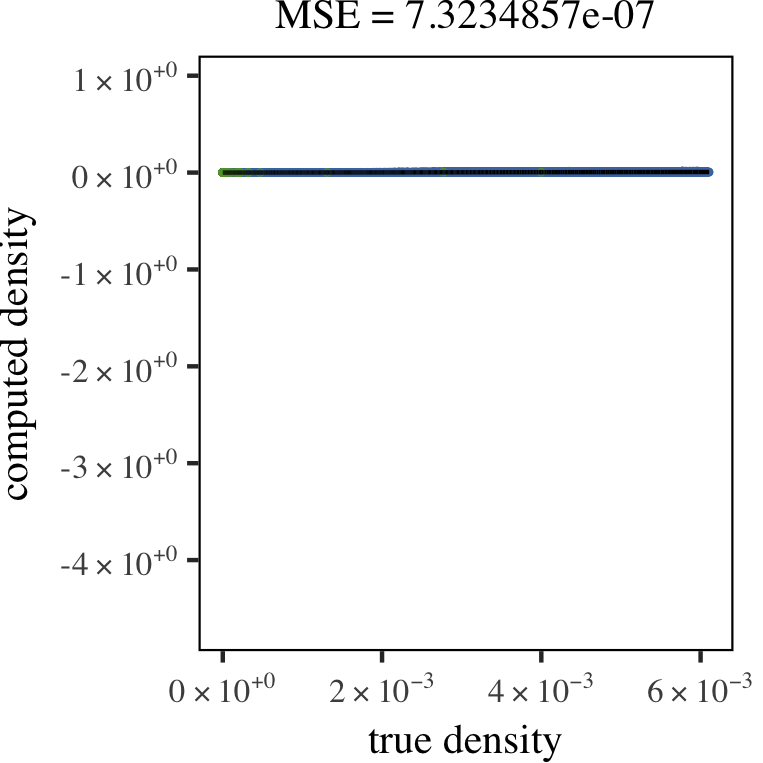
\includegraphics[keepaspectratio=true, width=\textwidth, height=0.23\textheight]{result/img/all/results_baakman_4_60000_mbe_silverman}
	\caption{Set \baakmanFour, \mbe}
	\label{fig:4:results:mbe:baakman4}
\end{subfigure}	
% Baakman 5 - MBE
\begin{subfigure}{0.23\textwidth}
	\centering
	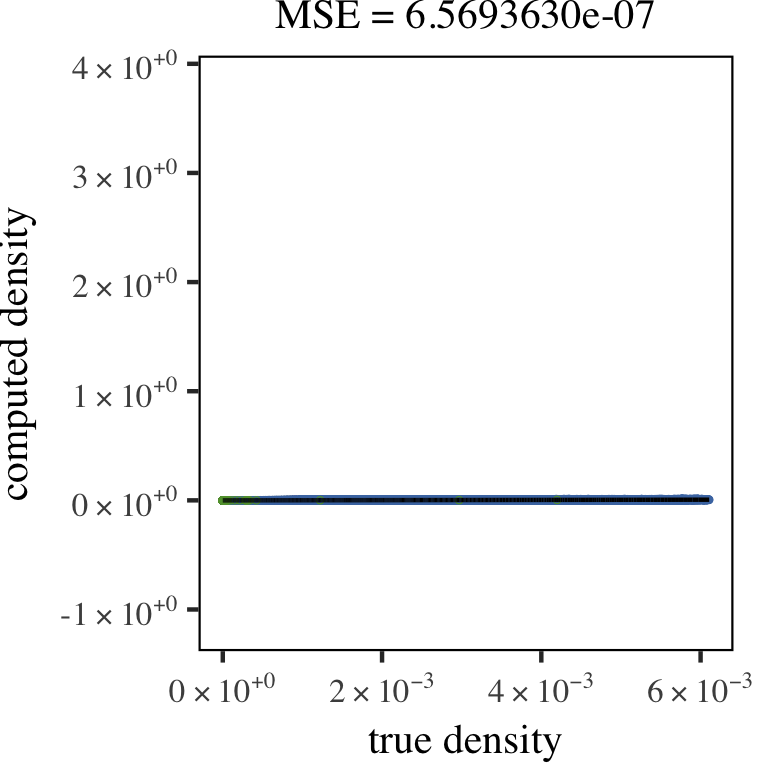
\includegraphics[keepaspectratio=true, width=\textwidth, height=0.23\textheight]{result/img/all/results_baakman_5_60000_mbe_silverman}
	\caption{Set \baakmanFive, \mbe}
	\label{fig:4:results:mbe:baakman5}
\end{subfigure}
% Ferdosi 1 - SAMBE
\begin{subfigure}{0.23\textwidth}
	\centering
	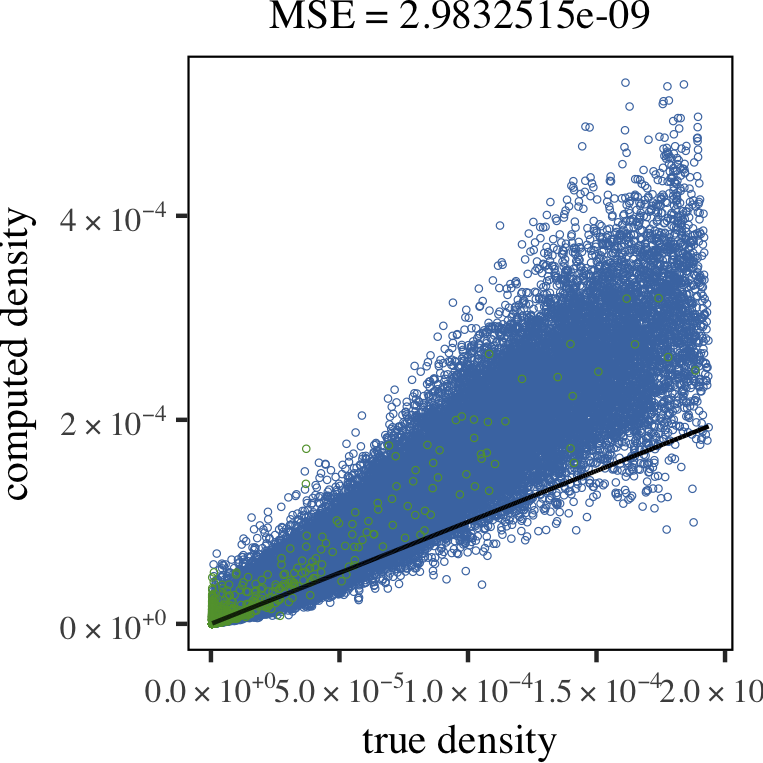
\includegraphics[keepaspectratio=true, width=\textwidth, height=0.23\textheight]{result/img/all/results_ferdosi_1_60000_sambe_silverman}
	\caption{Set \ferdosiOne, \sambe}
	\label{fig:4:results:sambe:ferdosi1}
\end{subfigure}
% Baakman 1	- SAMBE
\begin{subfigure}{0.23\textwidth}
	\centering
	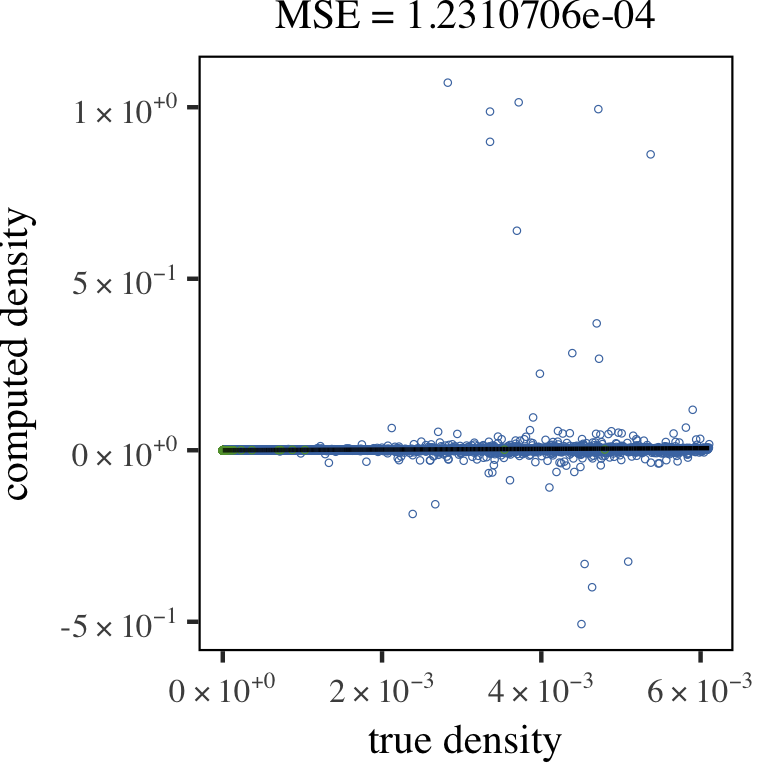
\includegraphics[keepaspectratio=true, width=\textwidth, height=0.23\textheight]{result/img/all/results_baakman_1_60000_sambe_silverman}
	\caption{Set \baakmanOne, \sambe}
	\label{fig:4:results:sambe:baakman1}
\end{subfigure}
% Baakman 4 - SAMBE
\begin{subfigure}{0.23\textwidth}
	\centering
	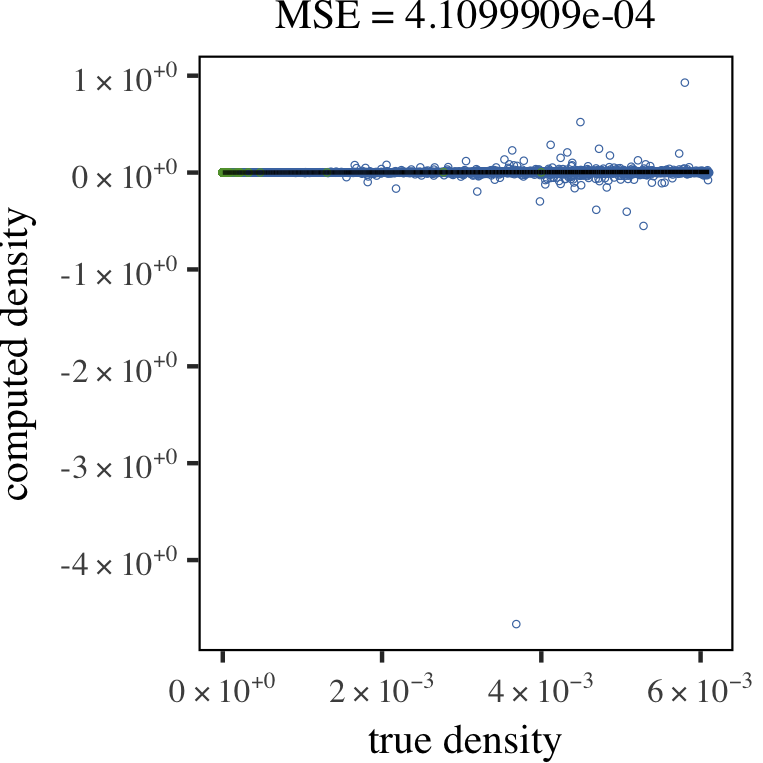
\includegraphics[keepaspectratio=true, width=\textwidth, height=0.23\textheight]{result/img/all/results_baakman_4_60000_sambe_silverman}
	\caption{Set \baakmanFour, \sambe}
	\label{fig:4:results:sambe:baakman4}
\end{subfigure}		
% Baakman 5 - SAMBE
\begin{subfigure}{0.23\textwidth}
	\centering
	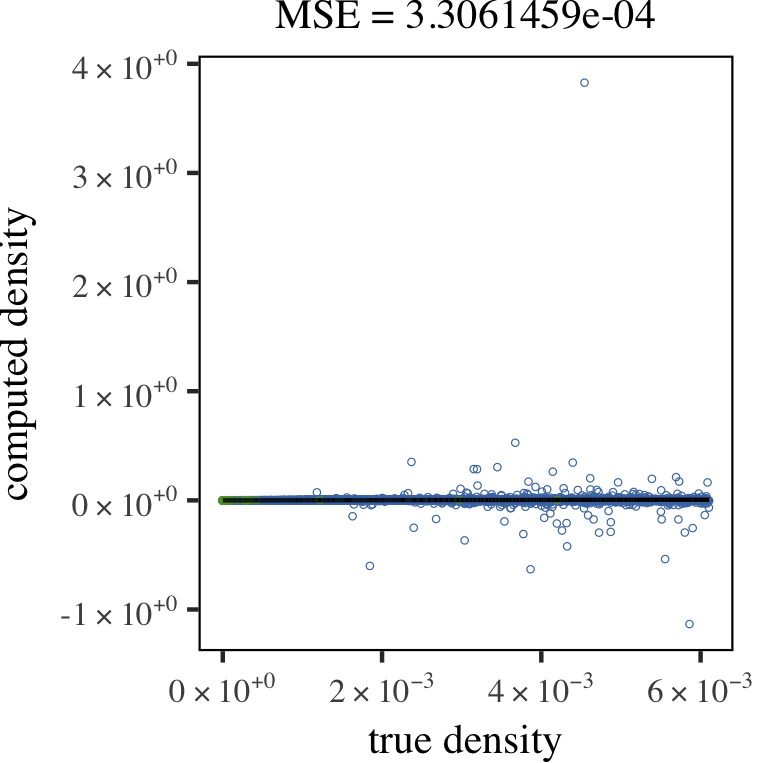
\includegraphics[keepaspectratio=true, width=\textwidth, height=0.23\textheight]{result/img/all/results_baakman_5_60000_sambe_silverman}
	\caption{Set \baakmanFive, \sambe}
	\label{fig:4:results:sambe:baakman5}
\end{subfigure}	
	\caption{Comparative plots for dataset \ferdosiOne, \baakmanOne, \baakmanFour, \baakmanFive.}
	\label{fig:4:results:singleSphere}
\end{figure*}

	\Cref{fig:4:results:singleSphere} presents the results of using the Modified Breiman Estimator and its shape adaptive variant to estimate the densities of the datasets in \cref{tab:3:simulated:datasets} that contain a single Gaussian distribution. 

% Ferdosi 1
	\Cref{fig:4:results:mbe:ferdosi1} confirms our findings from \cref{s:results:mse}, namely that the Modified Breiman Estimator gives a good approximation of the densities. The estimated densities both over, and undershoot the true density. \Cref{fig:4:results:mbe:ferdosi1}, on the other hand, shows that shape adaptive \mbe consistently overshoots the true density. 

% Baakman 1
	% Normal Plot
	Comparing the performance of the two estimators on dataset \baakmanOne with \crefrange{fig:4:results:mbe:baakman1}{fig:4:results:sambe:baakman1} we find that the Modified Breiman Estimator outperforms the shape-adaptive variant. The second estimator has some extreme outliers, the most extreme of which are \num{1.071674654143224}, and \num{-0.506829052779317}. 
	% No Outlier Plot
	Plotting only the results where the density as estimated by \sambe are in the range $\left(\num{0.0}, \num[round-precision=1]{0.07} \right)$ results in \Cref{fig:results:baakman1:noOutliers}. Observing \cref{fig:results:baakman1::noOUtliers:sambe} we find that using \sambe results in a greater spread of densities, but that the densities within the range $\left(\num[round-precision=1]{0.0}, \num[round-precision=1]{0.07} \right)$ reasonable approximate the true density.
	\begin{figure}[!ht]
		\centering
		\begin{subfigure}{0.6\columnwidth}
			\centering
			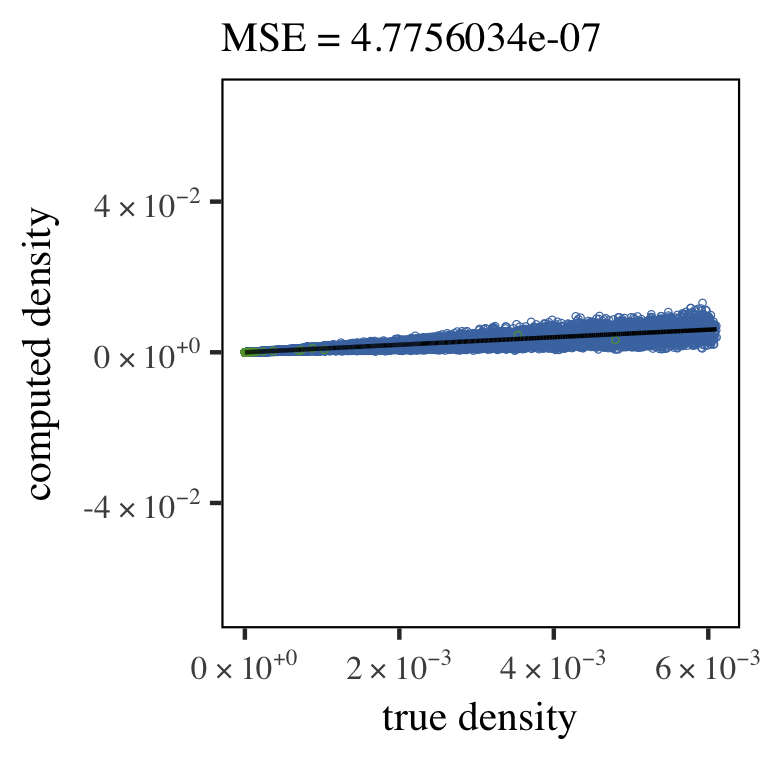
\includegraphics[width=\textwidth]{4/img/noOutliers/results_baakman_1_60000_mbe_silverman_no_outliers.png}
			\caption{\mbe}
			\label{fig:results:baakman1:noOutliers:mbe}
		\end{subfigure}
		\begin{subfigure}{0.6\columnwidth}
			\centering
			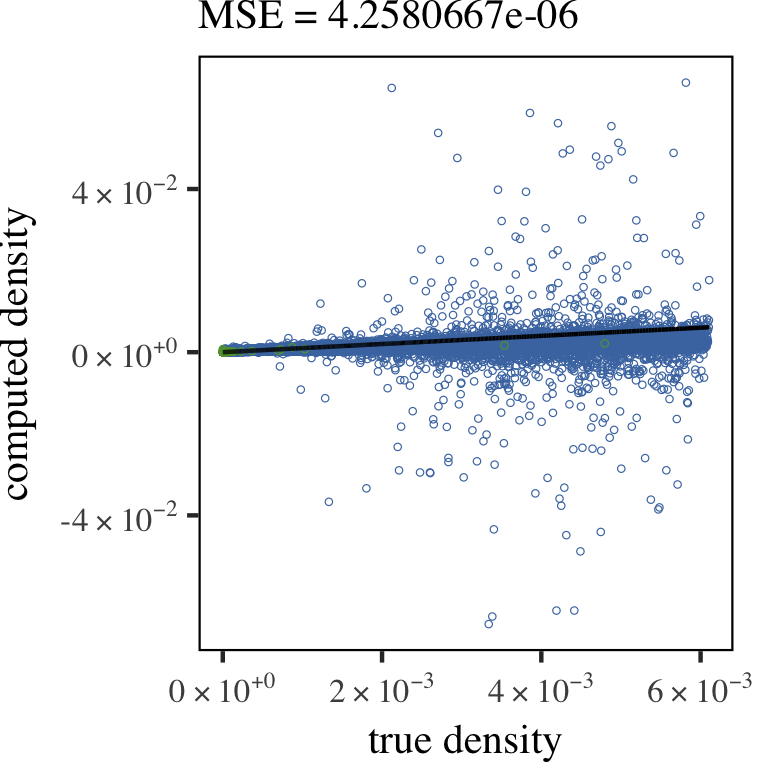
\includegraphics[width=\textwidth]{4/img/noOutliers/results_baakman_1_60000_sambe_silverman_no_outliers.png}
			\caption{\sambe}
			\label{fig:results:baakman1::noOUtliers:sambe}
		\end{subfigure}	
		\caption{Comparative plots between the true densities of dataset \baakmanOne as estimated by \subref{fig:results:baakman1:noOutliers:mbe} \mbe and \subref{fig:results:baakman1::noOUtliers:sambe} \sambe, with only the points whose density is estimated by \sambe to lie in $\left(\num{0.0}, \num[round-precision=1]{0.07} \right)$.}
		\label{fig:results:baakman1:noOutliers}
	\end{figure}

% Baakman 4
	% Normal Plot
	The results of data set \baakmanFour, shown in \crefrange{fig:4:results:mbe:baakman1}{fig:4:results:sambe:baakman1} are comparable to those of \baakmanOne: the original estimator approximates the density pretty well, the shape-adaptive variant has some extreme outliers, the densities estimated by \sambe fall in the range, $\left[\num{-4.660977565610216}, \num{0.928287124473193}\right]$, whereas the true densities all lie within $\left[\num{0.000000500000000}, \num{0.006107784664258}\right]$.
	% No Outlier Plot
	\Cref{fig:results:baakman4:noOutliers} presents the comparative plots for \mbe and \sambe for dataset \baakmanFour where patterns whose density was estimated to be outside the range $\left(\num{0.0}, \num[round-precision=2]{0.15} \right)$ are discarded. The results illustrated in this figure are comparable to those of \cref{fig:results:baakman1:noOutliers}: for a number of points the densities are overestimated, but otherwise the estimated densities seem reasonable.	

	\begin{figure}
		\centering
		\begin{subfigure}{0.6\columnwidth}
			\centering
			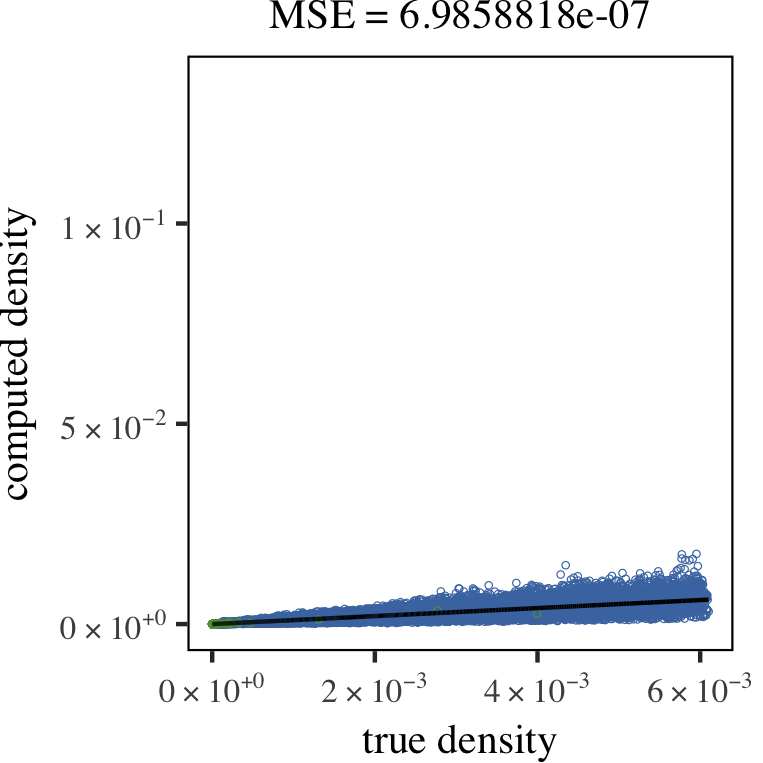
\includegraphics[width=\textwidth]{4/img/noOutliers/results_baakman_4_60000_mbe_silverman_no_outliers.png}
			\caption{\mbe}
			\label{fig:results:baakman4:noOutliers:mbe}
		\end{subfigure}
		\begin{subfigure}{0.6\columnwidth}
			\centering
			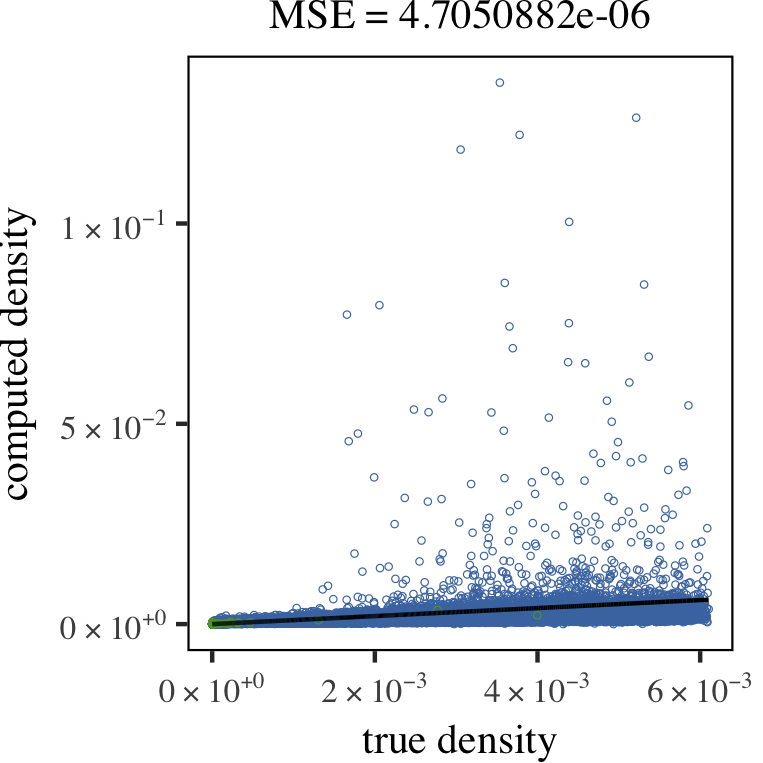
\includegraphics[width=\textwidth]{4/img/noOutliers/results_baakman_4_60000_sambe_silverman_no_outliers.png}
			\caption{\sambe}
			\label{fig:results:baakman4:noOUtliers:sambe}
		\end{subfigure}	
		\caption{Comparative plots between the true densities of dataset \baakmanFour as estimated by \subref{fig:results:baakman4:noOutliers:mbe} \mbe and \subref{fig:results:baakman4:noOUtliers:sambe} \sambe, with only the points whose density is estimated by \sambe to lie in $\left(\num{0.0}, \num{0.15} \right)$.}
		\label{fig:results:baakman4:noOutliers}
	\end{figure}

% Baakman 5
	% Normal Plot
	\Crefrange{fig:4:results:mbe:baakman5}{fig:4:results:sambe:baakman5} compares the performance of \mbe with \sambe on data set \baakmanFive. We once again observe that the shape adaptive variant results in extreme outliers, and that the non-shape adaptive estimator approximates the known densities pretty well. Whereas the shape-adaptive estimator returns pretty extreme results with densities estimated to be as high as \num{3.827317431934174} and as low as \num{-1.133853887375073}.
	%OutlierPlot
	Removing all patterns which have a density that is estimated by \sambe to lie outside the range $\left(\num{0.0}, \num[round-precision=2]{0.3} \right)$ results in \cref{fig:results:baakman5:noOutliers}. Comparing \cref{fig:results:baakman5:noOutliers:mbe} with \cref{fig:results:baakman5:noOUtliers:sambe} leads to the same conclusion as drawn about dataset \baakmanOne and \baakmanFour.

	\begin{figure}
		\centering
		\begin{subfigure}{0.6\columnwidth}
			\centering
			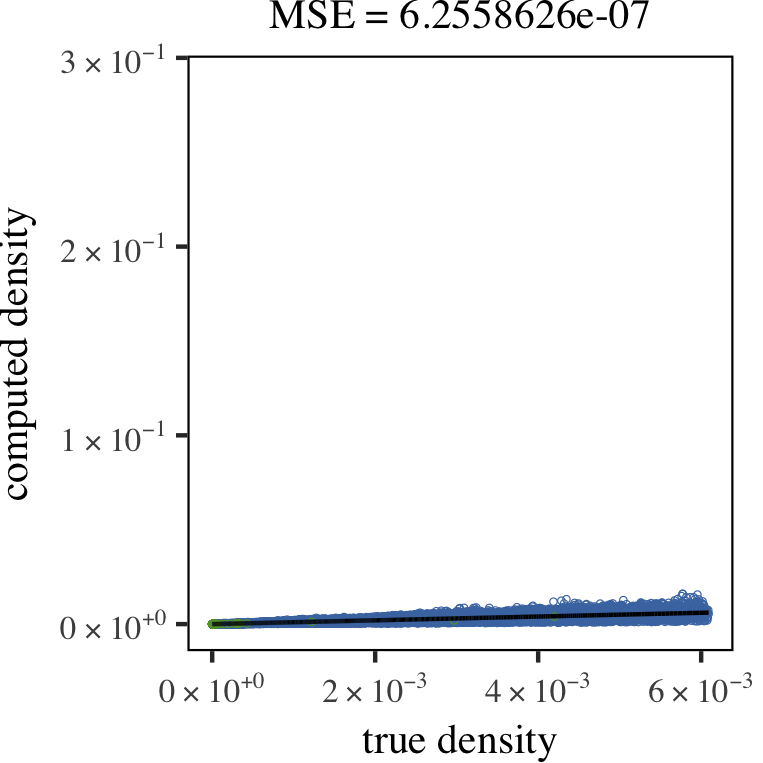
\includegraphics[width=\textwidth]{4/img/noOutliers/results_baakman_5_60000_mbe_silverman_no_outliers.png}
			\caption{\mbe}
			\label{fig:results:baakman5:noOutliers:mbe}
		\end{subfigure}
		\begin{subfigure}{0.6\columnwidth}
			\centering
			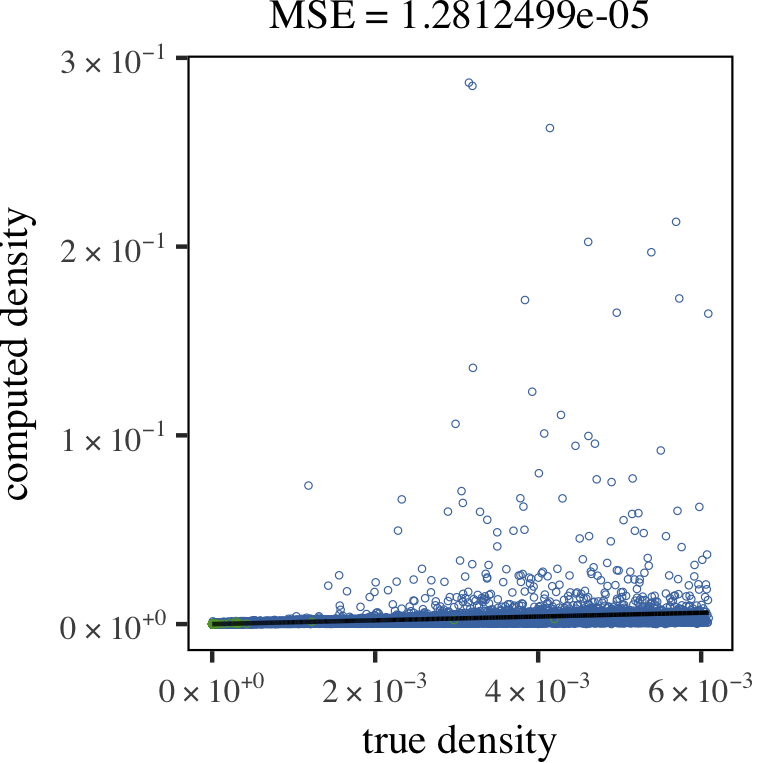
\includegraphics[width=\textwidth]{4/img/noOutliers/results_baakman_5_60000_sambe_silverman_no_outliers.png}
			\caption{\sambe}
			\label{fig:results:baakman5:noOUtliers:sambe}
		\end{subfigure}	
		\caption{Comparative plots between the true densities of dataset \baakmanFive as estimated by \subref{fig:results:baakman5:noOutliers:mbe} \mbe and \subref{fig:results:baakman5:noOUtliers:sambe} \sambe, with only the points whose density is estimated by \sambe to lie in $\left(\num{0.0}, \num{0.15} \right)$.}
		\label{fig:results:baakman5:noOutliers}
	\end{figure}

% Algehele observatie voor single sphere datsets
	% MBE beter dan SAMBE
	In general we have found that the Modified Breiman estimator works pretty well for data sets that contain a single Gaussian, especially if the Gaussian is spherical. Since the mean square error of the \mbe is lower for dataset \baakmanFive, than for dataset \baakmanFour how elongated the sphere is does not seem to influence the performance of this estimator. 
	% Hoe elongated heeft geen invloed
	The shape adaptive \mbe results in some extremely high and low values if it is used to estimate the densities of elongated Gaussians, when applied to a spherical Gaussians it overestimates the densities. The value of these extreme `densities' does not seem to be influenced by how elongated the Gaussian distribution is. 
	% Removing OUtliers
		\caption{Comparative plots for dataset \ferdosiOne, \baakmanOne, \baakmanFour, \baakmanFive.}
		\label{fig:4:results:singleSphere}
	\end{figure*}

	\Cref{fig:4:results:singleSphere} presents the results of using the Modified Breiman Estimator and its shape adaptive variant to estimate the densities of the datasets in \cref{tab:3:simulated:datasets} that contain a single Gaussian distribution. 

	% Ferdosi 1
		\Cref{fig:4:results:mbe:ferdosi1} confirms our findings from \cref{s:results:mse}, namely that the Modified Breiman Estimator gives a good approximation of the densities. The estimated densities both over, and undershoot the true density. \Cref{fig:4:results:mbe:ferdosi1}, on the other hand, shows that shape adaptive \mbe consistently overshoots the true density. 

	% Baakman 1
		% Normal Plot
		Comparing the performance of the two estimators on dataset \numberstringnum{\baakmanOneNum} with \crefrange{fig:4:results:mbe:baakman1}{fig:4:results:sambe:baakman1} we find that the Modified Breiman Estimator outperforms the shape-adaptive variant. The second estimator has some extreme outliers, the most extreme of which are \num{1.071674654143224}, and \num{-0.506829052779317}. 
		% No Outlier Plot
		Plotting only the results where the density as estimated by \sambe is in the range $\left(\num{0}, \num[round-precision=1]{0.07} \right)$ results in \Cref{fig:results:baakman1:noOutliers}The mean square errors of this subset are \num{4.6503038e-07} and \num{2.5008207e-06} for \mbe and \sambe, respectively. Observing \cref{fig:results:baakman1::noOUtliers:sambe} we find that using \sambe results in a greater spread of densities, but that the densities within the range $\left(\num[round-precision=1]{0.0}, \num[round-precision=1]{0.07} \right)$ reasonable approximate the true density.

		\begin{figure}
			\centering
			\begin{subfigure}{0.7\columnwidth}
				\centering
				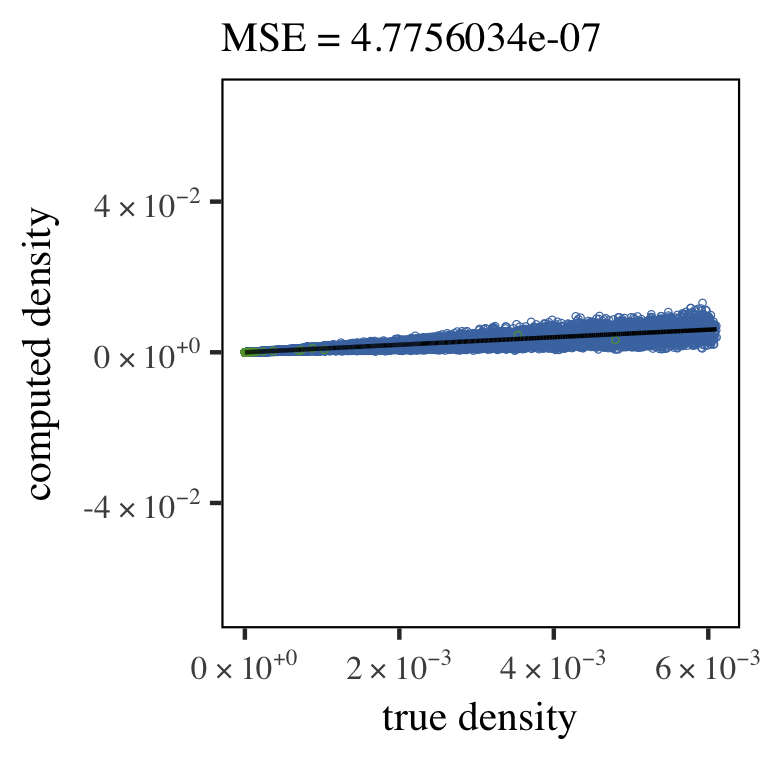
\includegraphics[width=\textwidth]{4/img/noOutliers/results_baakman_1_60000_mbe_silverman_no_outliers.png}
				\caption{\mbe}
				\label{fig:results:baakman1:noOutliers:mbe}
			\end{subfigure}
			\begin{subfigure}{0.7\columnwidth}
				\centering
				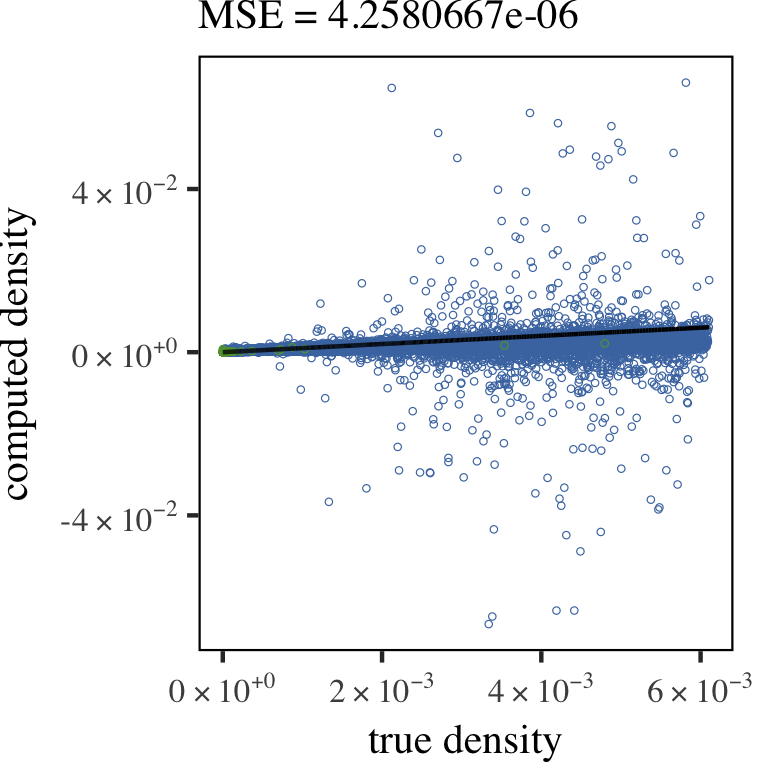
\includegraphics[width=\textwidth]{4/img/noOutliers/results_baakman_1_60000_sambe_silverman_no_outliers.png}
				\caption{\sambe}
				\label{fig:results:baakman1::noOUtliers:sambe}
			\end{subfigure}	
			\caption{Comparative plots between the true densities of dataset \baakmanOne as estimated by \subref{fig:results:baakman1:noOutliers:mbe} \mbe and \subref{fig:results:baakman1::noOUtliers:sambe} \sambe, with only the points whose density is estimated by \sambe to lie in $\left(\num{0}, \num[round-precision=1]{0.07} \right)$.}
			\label{fig:results:baakman1:noOutliers}
		\end{figure}

	% Baakman 4
		% Normal Plot
		The results of data set \numberstringnum{\baakmanFourNum}, shown in \crefrange{fig:4:results:mbe:baakman1}{fig:4:results:sambe:baakman1} are comparable to those of \numberstringnum{\baakmanOneNum}: the original estimator approximates the density pretty well, the shape-adaptive variant has some extreme outliers.
		\todo[inline]{Extra plaatje met de outliers eruit gehaald, kijken wat het dan geeft.}
		% No Outlier Plot
		\todo[inline]{Discuss outlier plots}
		% minimum original \num{-4.660977565610216}, maximum original \num{0.928287124473193}		

		\begin{figure}
			\centering
			\begin{subfigure}{0.7\columnwidth}
				\centering
				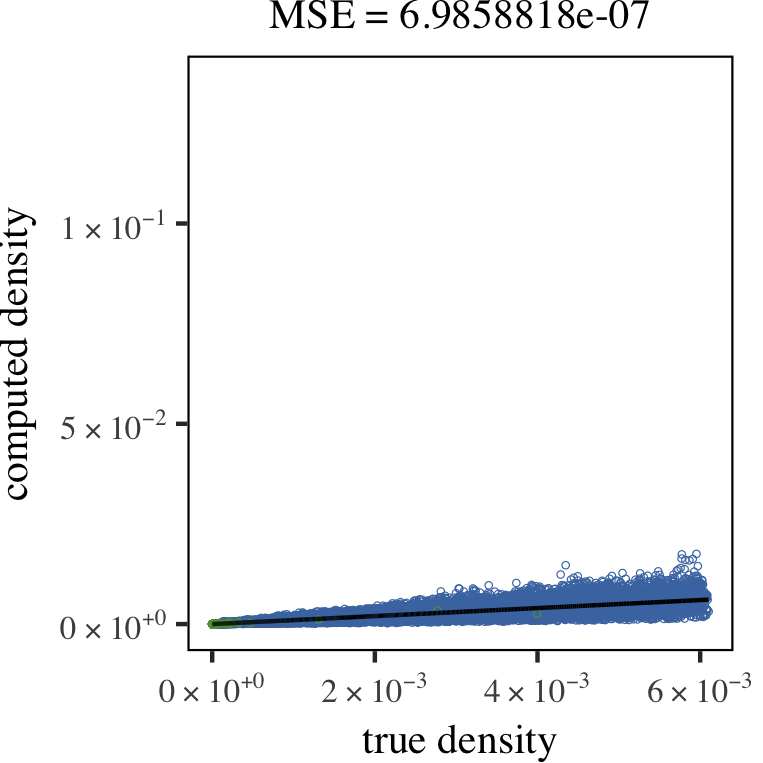
\includegraphics[width=\textwidth]{4/img/noOutliers/results_baakman_4_60000_mbe_silverman_no_outliers.png}
				\caption{\mbe}
				\label{fig:results:baakman4:noOutliers:mbe}
			\end{subfigure}
			\begin{subfigure}{0.7\columnwidth}
				\centering
				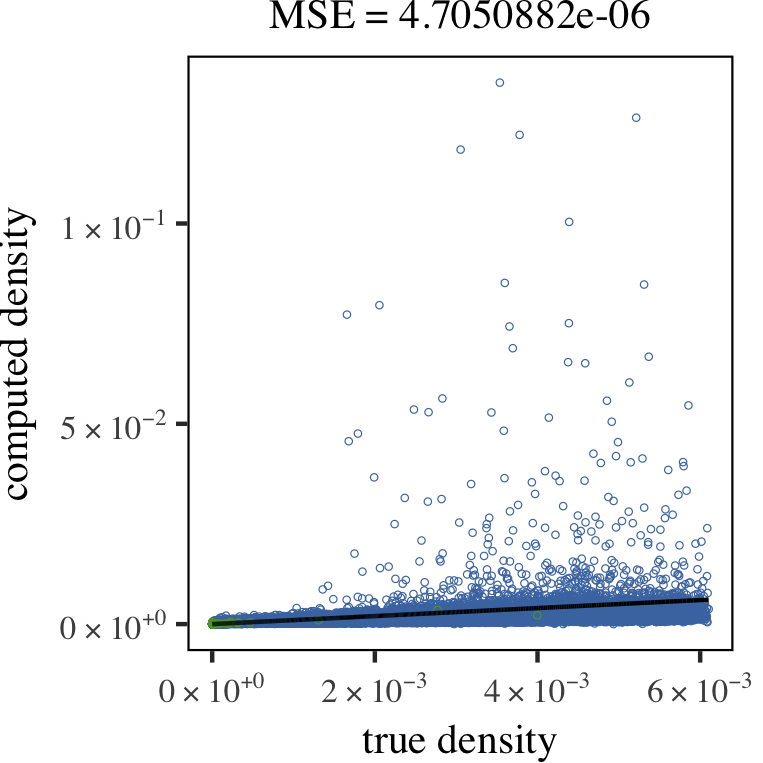
\includegraphics[width=\textwidth]{4/img/noOutliers/results_baakman_4_60000_sambe_silverman_no_outliers.png}
				\caption{\sambe}
				\label{fig:results:baakman4:noOUtliers:sambe}
			\end{subfigure}	
			\caption{Comparative plots between the true densities of dataset \baakmanFour as estimated by \subref{fig:results:baakman4:noOutliers:mbe} \mbe and \subref{fig:results:baakman4:noOUtliers:sambe} \sambe, with only the points whose density is estimated by \sambe to lie in $\left(\num{-0.15}, \num{0.15} \right)$.}
			\label{fig:results:baakman4:noOutliers}
		\end{figure}


	% Baakman 5
		\Crefrange{fig:4:results:mbe:baakman5}{fig:4:results:sambe:baakman5} compares the performance of \mbe with \sambe on data set \numberstringnum{\baakmanFiveNum}. We once again observe that the shape adaptive variant results in extreme outliers, and that the non-shape adaptive estimator approximates the known densities pretty well. 
		\todo[inline]{Extra plaatje met de outliers eruit gehaald, kijken wat het dan geeft.}

	% Algehele observatie voor single sphere datsets
		In general we have found that the Modified Breiman estimator works pretty well for data sets that contain a single Gaussian, especially if the Gaussian is spherical. Since the mean square error of the \mbe is lower for dataset \baakmanFive, than for dataset \baakmanFour how elongated the sphere is does not seem to influence the performance of this estimator. 
		%
		The shape adaptive \mbe results in some extremely high and low values if it is used to estimate the densities of elongated Gaussians, when applied to a spherical Gaussians it overestimates the densities. The value of these extreme `densities' does not seem to be influenced by how elongated the Gaussian distribution is.


% Multi Sphere Data
	\begin{figure*}
		\centering
		%!TEX root = ../paper.tex

% Ferdosi 2
\begin{subfigure}{0.23\textwidth}
	\centering
	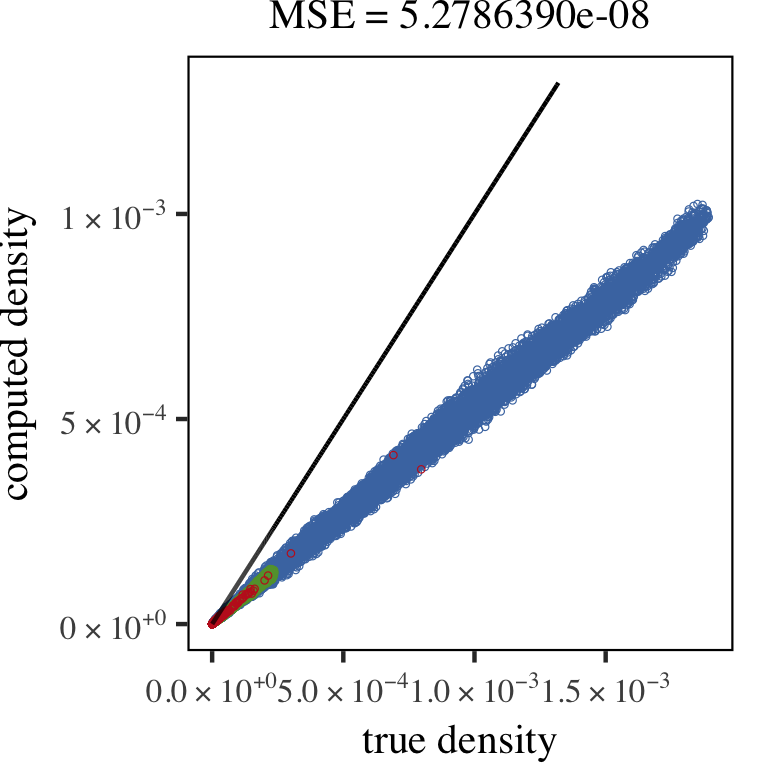
\includegraphics[keepaspectratio=true, width=\textwidth, height=0.23\textheight]{4/img/all/results_ferdosi_2_60000_mbe_silverman}
	\caption{Set \ferdosiTwo, \mbe}
	\label{fig:4:results:mbe:ferdosi2}
\end{subfigure}
\begin{subfigure}{0.23\textwidth}
	\centering
	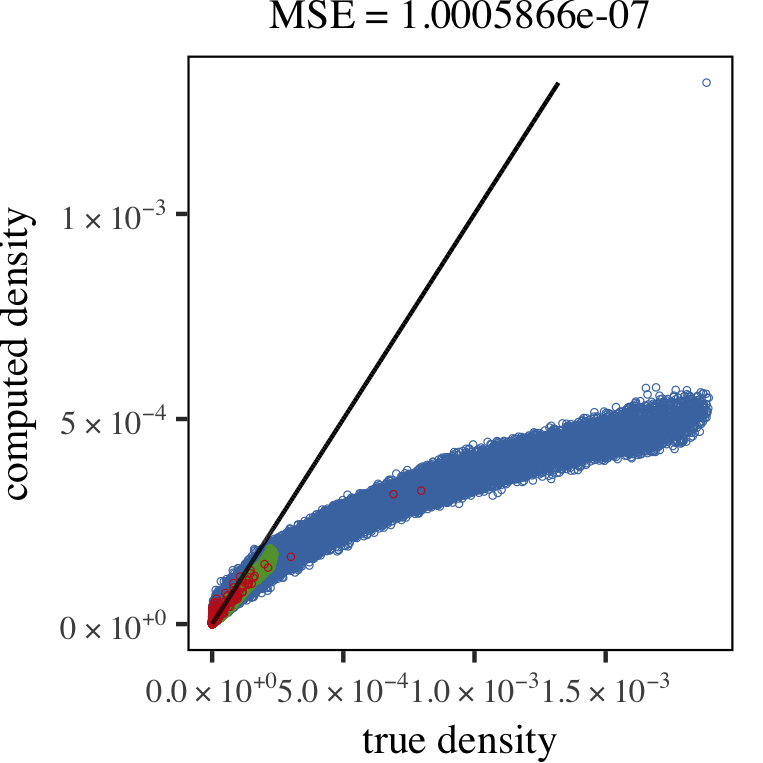
\includegraphics[keepaspectratio=true, width=\textwidth, height=0.23\textheight]{4/img/all/results_ferdosi_2_60000_sambe_silverman}
	\caption{Set \ferdosiTwo, \sambe}
	\label{fig:4:results:sambe:ferdosi2}
\end{subfigure}
% Baakman 2
\begin{subfigure}{0.23\textwidth}
	\centering
	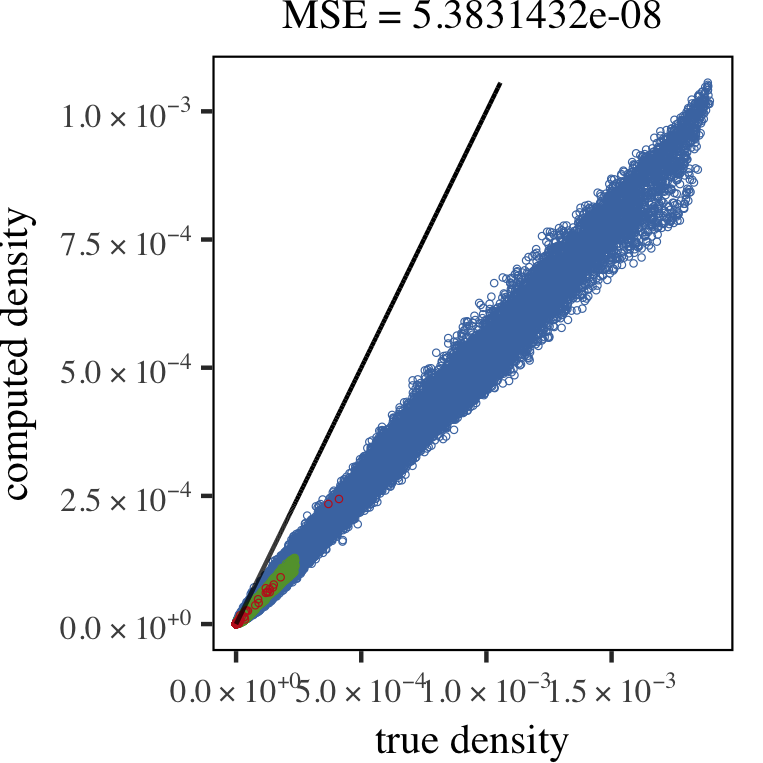
\includegraphics[keepaspectratio=true, width=\textwidth, height=0.23\textheight]{4/img/all/results_baakman_2_60000_mbe_silverman}
	\caption{Set \baakmanTwo, \mbe}
	\label{fig:4:results:mbe:baakman2}
\end{subfigure}
\begin{subfigure}{0.23\textwidth}
	\centering
	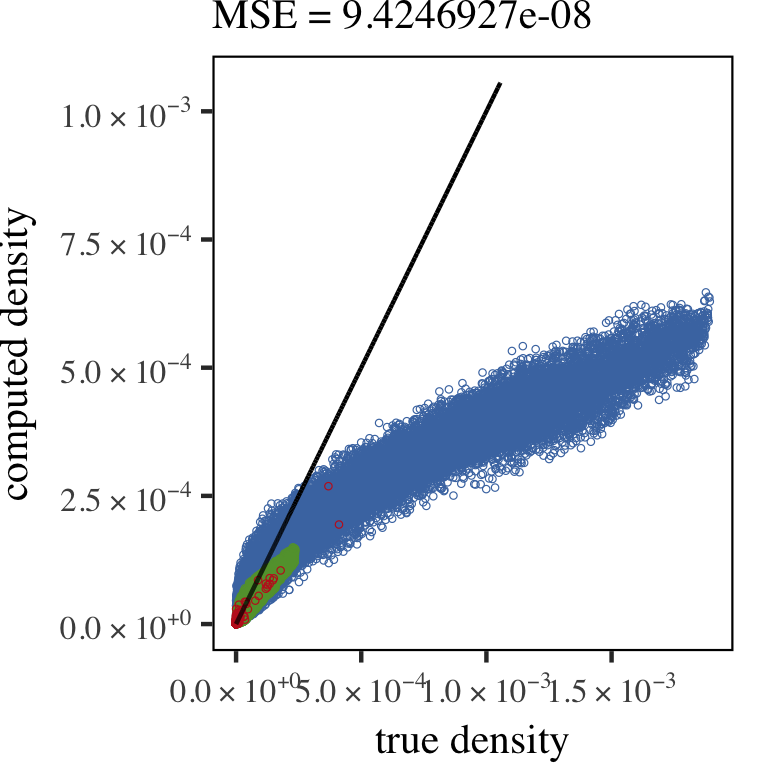
\includegraphics[keepaspectratio=true, width=\textwidth, height=0.23\textheight]{4/img/all/results_baakman_2_60000_sambe_silverman}
	\caption{Set \baakmanTwo, \sambe}
	\label{fig:4:simulated:datasets:sambe:baakman2}
\end{subfigure}
% Ferdosi 3
\begin{subfigure}{0.23\textwidth}
	\centering
	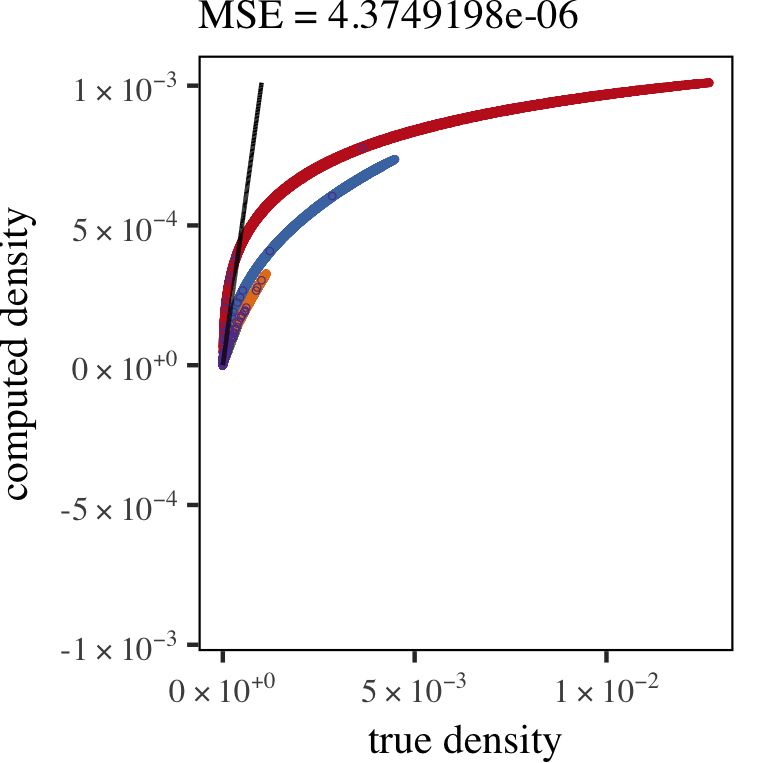
\includegraphics[keepaspectratio=true, width=\textwidth, height=0.23\textheight]{4/img/all/results_ferdosi_3_120000_mbe_silverman.png}
	\caption{Set \ferdosiThree, \mbe}
	\label{fig:4:results:mbe:ferdosi3}
\end{subfigure}
\begin{subfigure}{0.23\textwidth}
	\centering
	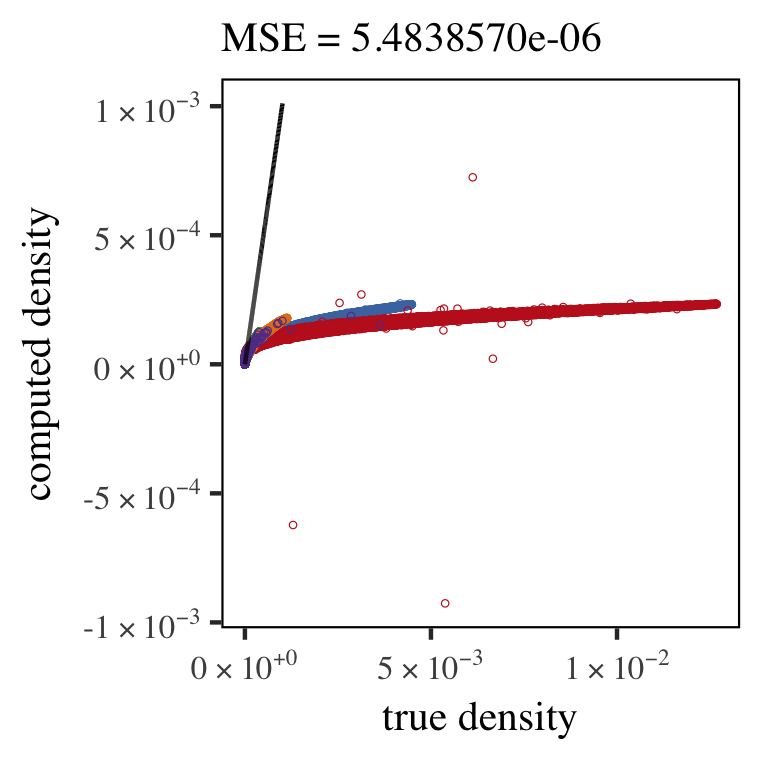
\includegraphics[keepaspectratio=true, width=\textwidth, height=0.23\textheight]{4/img/all/results_ferdosi_3_120000_sambe_silverman}
	\caption{Set \ferdosiThree, \sambe}
	\label{fig:4:simulated:datasets:sambe:ferdosi3}
\end{subfigure}
% Baakman 3
\begin{subfigure}{0.23\textwidth}
	\centering
	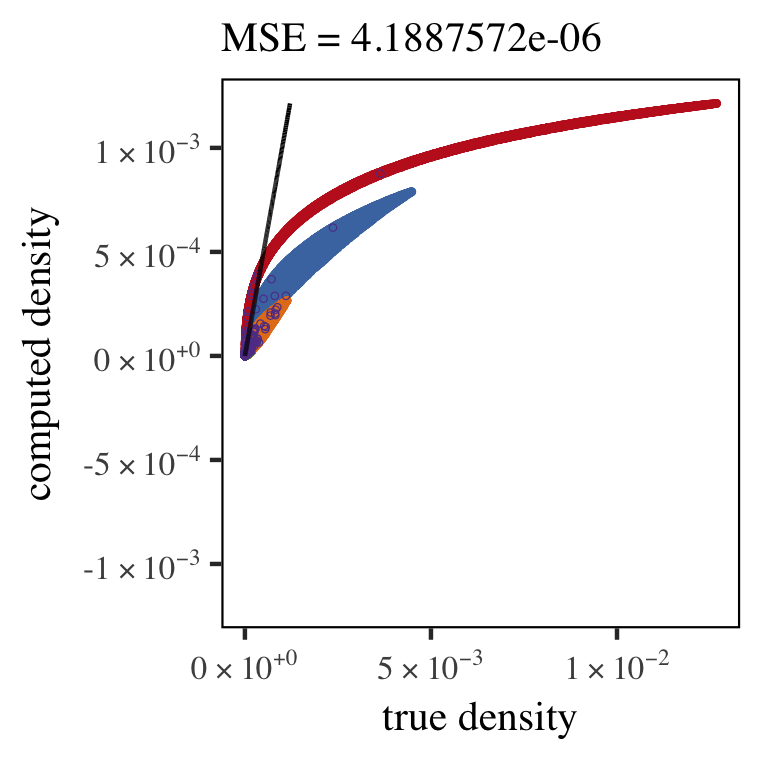
\includegraphics[keepaspectratio=true, width=\textwidth, height=0.23\textheight]{4/img/all/results_baakman_3_120000_mbe_silverman}
	\caption{Set \baakmanThree, \mbe}
	\label{fig:4:results:mbe:baakman3}
\end{subfigure}	
\begin{subfigure}{0.23\textwidth}
	\centering
	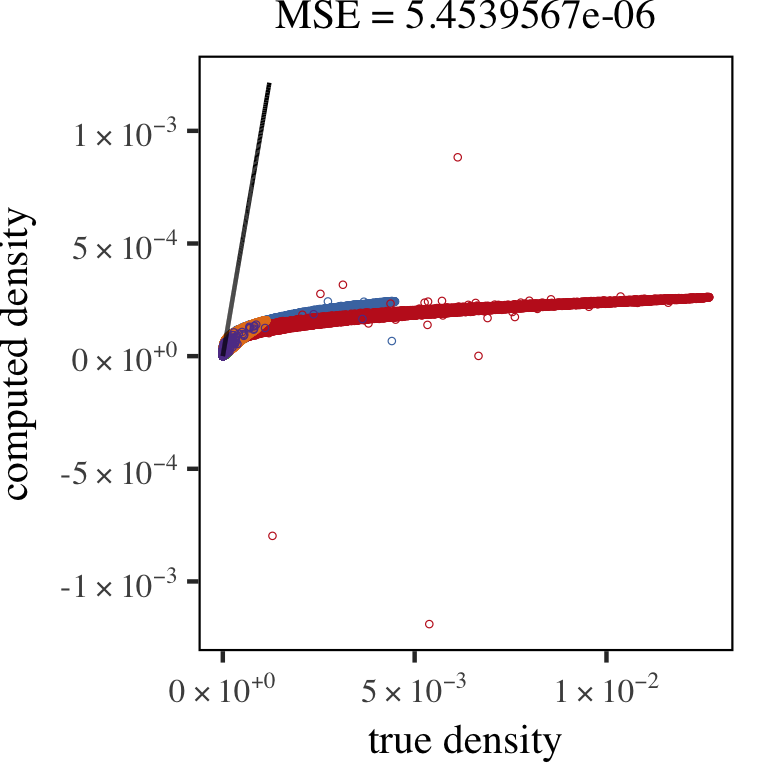
\includegraphics[keepaspectratio=true, width=\textwidth, height=0.23\textheight]{4/img/all/results_baakman_3_120000_sambe_silverman}
	\caption{Set \baakmanThree, \sambe}
	\label{fig:4:results:sambe:baakman3}
\end{subfigure}	
		\caption{Comparative plots for dataset \ferdosiTwo, \ferdosiThree, \baakmanTwo, \baakmanThree.}
		\label{fig:4:resuts:multiSphere}
	\end{figure*}

	\todo[inline]{What do we observe for dataset ferdosi 2, baakman 2, ferdosi 3, baakman 3}
